\chapter{Interface}
\section{Affichage 3D}
Nos recherches sur la façon de réaliser un rendu 3D en Java nous a amené à utiliser une bibliothèque : \textit{Java3D}\cite{cite5}.
Même si le rendu à un instant t est satisfaisant (voir image ci-dessous), il ne nous permet pas, du moins de façon optimisée, de réaliser des animations comme la rotation du cube, le rendu étant figé une fois affiché.
\begin{figure}[h]
\begin{center}
	\makebox[\textwidth]{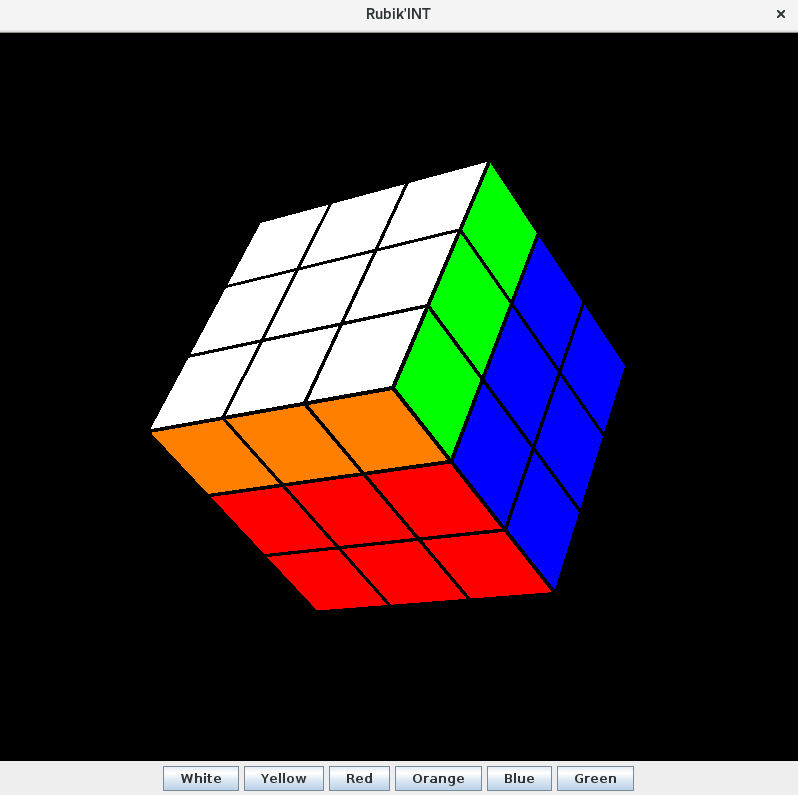
\includegraphics[width=.4\paperwidth]{diagrammes/rendu3D.png}}
\end{center}
\caption{GUI}
\end{figure}
Cet essai nous a permis de mieux cerner notre besoin. 
Il est nécessaire d'avoir un rendu 3D dans lequel l'objet affiché reste modifiable, dans notre cas de pouvoir réaliser les animation de rotation du cube. C'est pourquoi nous avons finalement décidé de réaliser tout cela à l'aide de la bibliothèque : \textit{OpenGL}\cite{cite6}.

\section{Interface fenêtrée}
Cet affichage 3D devra être intégré dans une interface, il sera accompagné de boutons pour rendre notre programme de résolution autonome et facile d'utilisation. Nous pouvons voir une ébauche d'utilisation de la bibliothèque \textit{Swing}\cite{cite9} sur la photo ci-dessus. L'objectif de cette première fenêtre est de faire tourner la face du cube de la couleur associée au bouton lorsque l'utilisateur clique dessus.

À terme, l'interface sera scindée en trois parties selon la logique suivante :

\begin{itemize}
    \item Un accueil pour que l'utilisateur puisse choisir la façon dont il veut résoudre son Rubik's cube (avec ou sans prise de photo d'un vrai cube)
    \item Une interface permettant la prise de photo du cube et donc de récupérer sa configuration 
    \item Une interface pour la résolution du cube.
\end{itemize}
Notre objectif est de rendre l'interface le plus \textit{user-friendly} possible.


